%% Technical Report for the work on the AI-DSL over the period of
%% March to May 2021.

\documentclass[]{report}
\usepackage{url}
\usepackage{minted}
\usepackage[textsize=footnotesize]{todonotes}
\newcommand{\kabir}[2][]{\todo[color=yellow,author=kabir, #1]{#2}}
\newcommand{\nil}[2][]{\todo[color=purple,author=nil, #1]{#2}}
\usepackage{hyperref}
\usepackage{listings}
\lstset{basicstyle=\ttfamily\footnotesize,breaklines=false,frame=single}
\usepackage{float}
\restylefloat{table}
\usepackage{graphicx}
\usepackage[font=small,labelfont=bf]{caption}
\usepackage{subcaption}

\begin{document}

\title{AI-DSL Technical Report (February to May 2021)}
\author{Nil Geisweiller, Kabir Veitas, Eman Shemsu Asfaw, Samuel Roberti}
\maketitle

\begin{abstract}
Based on~\cite{GoertzelGeisweillerBlog}.
\end{abstract}

\tableofcontents

\chapter{Nil's work}

Work done:
\begin{enumerate}
\item Implement \texttt{RealizedFunction} as described
  in~\cite{GoertzelGeisweillerBlog}.
\item Implement a network of trivially simple AI services implemented
  in Idris2, and use Idris compiler to type check if they can properly
  connect to each other.
\item Implement a Registry prototype, as a proof-of-concept for
  querying AI services based on their dependently typed
  specifications.
\end{enumerate}

\section{Realized Function}
\label{realized_function}

\subsection{Description}

The \texttt{RealizedFunction} data structure, as introduced
in~\cite{GoertzelGeisweillerBlog}, is a wrapper around a regular
function to integrate aspects of its specifications pertaining to its
execution on real physical substrates as opposed to just its
algorithmic properties.  For instance it contains descriptions of
costs (financial, computational, etc) and performances (quality, etc)
captured in the \texttt{RealizedAttributes} data structure, as
introduced in~\cite{GoertzelGeisweillerBlog} as well.

For that iteration we have implemented a simple version of
\texttt{RealizedFunction} and \texttt{RealizedAttributes} in
Idris2~\cite{Idris}.  The \texttt{RealizedAttributes} data structure
contains
\begin{itemize}
\item \texttt{Costs}: as a triple of three constants,
  \texttt{financial}, \texttt{temporal} and \texttt{computational},
\item \texttt{Quality}: as a single \texttt{quality} value.
\end{itemize}
as well as an example of compositional law,
\texttt{add\_costs\_min\_quality}, where costs are additive and
quality is infimumitive\nil{is there a word for that?}.  Below is a
small snippet of that code to give an idea of how it looks like

\begin{minted}[mathescape]{idris}
record RealizedAttributes where
  constructor MkRealizedAttributes
  costs : Costs
  quality : Quality
\end{minted}

\begin{minted}[mathescape]{idris}
add_costs_min_quality : RealizedAttributes ->
                        RealizedAttributes ->
                        RealizedAttributes
add_costs_min_quality f_attrs g_attrs = fg_attrs where
  fg_attrs : RealizedAttributes
  fg_attrs = MkRealizedAttributes (add_costs f_attrs.costs g_attrs.costs)
                                  (min f_attrs.quality g_attrs.quality)
\end{minted}
The full implementation can be found in
\href{https://github.com/singnet/ai-dsl/blob/master/experimental/realized-function/RealizedAttributes.idr}{RealizedAttributes.idr},
under the
\href{https://github.com/singnet/ai-dsl/blob/master/experimental/realized-function/}{experimental/realized-function/}
folder of the \href{https://github.com/singnet/ai-dsl/}{ai-dsl
  repository}~\cite{AIDSLRepo}.\\

Then we have implemented \texttt{RealizedFunction} that essentially
attaches a \texttt{RealizedAttributes} instance to a function.  In
addition we have implemented a composition (as in function
composition) operating on \texttt{RealizedFunction} instead of
regular function, making use of that compositional law above.
Likewise below is a snippet of that code

\begin{minted}[mathescape]{idris}
data RealizedFunction : (t : Type) -> (attrs : RealizedAttributes) -> Type where
  MkRealizedFunction : (f : t) -> (attrs : RealizedAttributes) ->
                       RealizedFunction t attrs
\end{minted}

\begin{minted}[mathescape]{idris}
compose : {a : Type} -> {b : Type} -> {c : Type} ->
          (RealizedFunction (b -> c) g_attrs) ->
          (RealizedFunction (a -> b) f_attrs) ->
          (RealizedFunction (a -> c) (add_costs_min_quality f_attrs g_attrs))
compose (MkRealizedFunction g g_attrs) (MkRealizedFunction f f_attrs) =
  MkRealizedFunction (g . f) (add_costs_min_quality f_attrs g_attrs)
\end{minted}
The full implementation can be found in
\href{https://github.com/singnet/ai-dsl/blob/master/experimental/realized-function/RealizedFunction.idr}{RealizedFunction.idr}
under the same folder.

\subsection{Objectives and achievements}

The objectives of this work was to see if Idris2 was able to type
check that the realized attributes of composed realized functions
followed the defined compositional law.  We have found that Idris2 is
not only able to do that, but to our surprise much faster that Idris1
(instantaneous instead of seconds to minutes), by bypassing induction
on numbers and using efficient function-driven rewriting on the
realized attributes instead.  That experiment can be found in
\href{https://github.com/singnet/ai-dsl/blob/master/experimental/realized-function/RealizedFunction-test.idr}{RealizedFunction-test.idr},
under the
\href{https://github.com/singnet/ai-dsl/blob/master/experimental/realized-function/}{experimental/realized-function/}
folder of the \href{https://github.com/singnet/ai-dsl/}{ai-dsl
  repository}~\cite{AIDSLRepo}.

\subsection{Future work}

Experimenting with constants as realized attributes was the first step
in our investigation.  The subsequent steps will be to replace
constants by functions, probability distributions and other
sophisticated ways to represent costs and quality.

\section{Network of Idris AI services}
\label{network_idris_ai_services}

\subsection{Description}

In this work we have implemented a small network of trivially simple
AI services, with the objective of testing if the Idris compiler could
be used to type check the validity of their connections. Three primary
services were implemented
\begin{enumerate}
\item \texttt{incrementer}: increment an integer by 1
\item \texttt{twicer}: multiply an integer by 2
\item \texttt{halfer}: divide an integer by 2
\end{enumerate}
as well as composite services based on these primary services, such as
\begin{itemize}
\item \texttt{incrementer . halfer . twicer}
\end{itemize}
with the objective of testing that such compositions were properly
typed.  The networking part was implemented based on the
SingularityNET example service~\cite{SNETExampleService} mentioned in
the SingularityNET tutorial~\cite{SNETTutorial}.  The specifics of
that implementation are of little importance for that report and thus
are largely ignored.  The point was to try to be as close as possible
to real networking conditions.  For the part that matters to us we may
mention that communications between AI services are handled by
gRPC~\cite{gRPC}, which has some level of type checking by insuring
that the data being exchanged fulfill some type structures (list of
integers, union type of string and bool, etc) specified in Protocol
Buffers~\cite{Protobuf}.  Thus one may see the usage of Idris in that
context as adding an enhanced refined verification layer on top of
gRPC making use of the expressive power of dependent types.

\subsection{Objectives and achievements}

As mentioned above the objectives of such an experiment was to see how
the Idris compiler can be used to type check combinations of AI
services.  It was initially envisioned to make use of dependent types
by specifying that the \texttt{twicer} service outputs an even
integer, as opposed to any integer, and that the \texttt{halfer}
service only accepts an even integer as well.  The idea was to
prohibit certain combinations such as
\begin{itemize}
\item \texttt{halfer . incrementer . twicer}
\end{itemize}
Since the output of \texttt{incrementer . twicer} is provably odd,
\texttt{halfer} should refuse it and such combination should be
rejected.  This objective was not reached in this experiment, but
similar objectives were reached other experiments, see Section
\ref{aidsl_registry}\nil{Add ref to Sam's work}.  The other objective
was to type check that the compositions have realized attributes
corresponding to the compositional law implemented in Section
\ref{realized_function}, which was fully achieved in this experiment.
For instance by changing either the types, costs or quality of the
following composition
\begin{minted}[mathescape]{idris}
-- Realized (twicer . incrementer).
rlz_compo1_attrs : RealizedAttributes
rlz_compo1_attrs = MkRealizedAttributes (MkCosts 300 30 3) 0.9
-- The following does not work because 301 /= 200+100
-- rlz_compo1_attrs = MkRealizedAttributes (MkCosts 301 30 3) 0.9
rlz_compo1 : RealizedFunction (Int -> Int) Compo1.rlz_compo1_attrs
rlz_compo1 = compose rlz_twicer rlz_incrementer
\end{minted}
defined in
\href{https://github.com/singnet/ai-dsl/blob/master/experimental/simple-idris-services/service/Compo1.idr}{experimental/simple-idris-services/service/Compo1.idr},
the corresponding service would raise a type checking error at start
up.  More details on the experiment and how to run it can be found in
the
\href{https://github.com/singnet/ai-dsl/blob/master/experimental/simple-idris-services/README.md}{\texttt{README.md}}
under the
\href{https://github.com/singnet/ai-dsl/blob/master/experimental/simple-idris-services/}{\texttt{experimental/simple-idris-services/service/}}
folder of the \href{https://github.com/singnet/ai-dsl/}{ai-dsl
  repository}~\cite{AIDSLRepo}.

\subsection{Future work}

Such experiment was good to explore how Idris can be integrated to a
network of services.  What we need to do next is experiment with
actual AIs algorithms, ideally making full use of dependent types in
their specifications.  Such endeavor was actually attempted by using
an existing set of cooperating AI services\nil{Ref to Kabir's fake
  news detector}, but it was eventually concluded to be too ambitious
for that iteration and was postponed for the next.

Obviously we want to be able to reuse existing AI services and write
their enhanced specifications on top of them, as opposed to writing
both specification and code in Idris/AI-DSL.  To that end it was noted
that having a Protobuf to/from Idris/AI-DSL converter would be useful,
so that a developer can start from an existing AI service, specified
in Protobuf, and enriched it with dependent types in Idris/AI-DSL.
The other way around could be useful as well to enable a developer to
implement AI services entirely in Idris/AI-DSL and expose their
Protobuf specification to the network.  To that end having an
implementation of gRPC for Idris/AI-DSL could be handy as well.

\section{AI-DSL Registry}
\label{aidsl_registry}

\subsection{Description}

One important goal of the AI-DSL is to have a system that can perform
autonomous matching and composition of AI services, so that provided
the specification of an AI, it should suffice to find it, complete it
or even entirely build it from scratch.  We have implemented a
proof-of-concept \emph{registry} to start experimenting with such
functionalities.

So far we have two versions in the
\href{https://github.com/singnet/ai-dsl/}{ai-dsl repository}, one
without dependent types support, under
\href{https://github.com/singnet/ai-dsl/blob/master/experimental/realized-function/}{experimental/registry/},
and a more recent one with dependent type support that can be found
under
\href{https://github.com/singnet/ai-dsl/blob/master/experimental/registry-dtl/}{experimental/registry-dtl/}.
We will focus our attention on the latter which is far more
interesting.\\

The AI-DSL registry (reminiscent of the SingularityNET
registry~\cite{TODO}) is itself an AI service with the following functions
\begin{enumerate}
\item \texttt{retrieve}: find AI services on the network fulfilling a
  given specification.
\item \texttt{compose}: construct composite services fulfilling that
  specification.  Useful when no such AI services can be found.
\end{enumerate}

The experiment contains the same \texttt{incrementer}, \texttt{twicer}
and \texttt{halfer} services described in Section
\ref{network_idris_ai_services} with the important distinction that
their specifications now utilize dependent types.  For instance the
type signature of \texttt{twicer} becomes
\begin{minted}[mathescape]{idris}
twicer : Integer -> EvenInteger
\end{minted}
instead of
\begin{minted}[mathescape]{idris}
twicer : Integer -> Integer
\end{minted}
where \texttt{EvenInteger} is actually a shorthand for the following
dependent type
\begin{minted}[mathescape]{idris}
EvenInteger : Type
EvenInteger = (n : WFInt ** Parity n 2)
\end{minted}
that is a \emph{dependent pair} composed of a \emph{well founded
integer} of type \texttt{WFInt} and a dependent data structure,
\texttt{Parity} containing a proof that the first element of the pair,
\texttt{n}, is even.  More details on that can be found in
Section\nil{Add ref to Sam's work}.

For now our prototype of AI-DSL registry implements the
\texttt{retreive} function, which, given an Idris type signature,
searches through a database of AI services and returns one fulfilling
that type.  In that experiment the database of AI services is composed
of \texttt{incrementer}, \texttt{twicer}, \texttt{halfer}, the
\texttt{registry} itself and \texttt{compo}, a composite service using
previously listed services.

One can query each service via gRPC.  For instance querying the
\texttt{retreive} function of the \texttt{registry} service with the
following input
\begin{minted}[mathescape]{idris}
String -> (String, String)
\end{minted}
outputs
\begin{minted}[mathescape]{idris}
Registry.retreive
\end{minted}
which is itself.  Likewise one can query
\begin{minted}[mathescape]{idris}
Integer -> Integer
\end{minted}
which outputs
\begin{minted}[mathescape]{idris}
Incrementer.incrementer
\end{minted}
corresponding to the \texttt{Incrementer} service with the
\texttt{incrementer} function.
Next one can provide a query involving dependent types, such as
\begin{minted}[mathescape]{idris}
Integer -> EvenInteger
\end{minted}
outputting
\begin{minted}[mathescape]{idris}
Twicer.twicer
\end{minted}
Or equivalently provide the unwrapped dependent type signature
\begin{minted}[mathescape]{idris}
Integer -> (n : WFInt ** Parity n (Nat 2))
\end{minted}
retrieving the correct service again
\begin{minted}[mathescape]{idris}
Twicer.twicer
\end{minted}

At the heart of it is Idris.  Behind the scene the registry
communicates the type signature to the Idris REPL and requests, via
the {\texttt :search} meta function, all loaded functions matching the
type signature.  Then the registry just returns the first match.

Secondly, we can now write composite services with missing parts.  The
\texttt{compo} service illustrates this.  This service essentially
implements the following composition
\begin{minted}[mathescape]{idris}
incrementer . halfer . (Registry.retrieve ?type)
\end{minted}
Thus upon execution queries the registry to fill the hole with the
correct, according to its specification, service.

More details about this, including steps to reproduce it all, can be
found in the
\href{https://github.com/singnet/ai-dsl/blob/master/experimental/registry-dsl/README.md}{\texttt{README.md}}
under the
\href{https://github.com/singnet/ai-dsl/blob/master/experimental/registry-dsl/}{\texttt{experimental/simple-idris-services/service/}}
folder of the \href{https://github.com/singnet/ai-dsl/}{ai-dsl
  repository}~\cite{AIDSLRepo}.

\subsection{Objectives and achievements}

As shown above we were able to implement a proof-of-concept of an
AI-DSL registry.  Only the \texttt{retrieve} function was implemented.
The \texttt{compose} function still remains to be implemented,
although the \texttt{compo} service is somewhat halfway there, with
limitations, for instance the missing type, \texttt{?type}, was
hardwired in the code, \texttt{Integer -> EvenInteger}.  It should be
noted however that Idris is in principle capable of inferring such
information but more work is needed to more fully explore that
functionality.

Of course it is a very simple example, in fact the simplest we could
come up with, but we believe serves as a nice proof-of-concept, and
demonstrates that AI services matching and such, using dependent types
as formal specification language, is possible.

\subsection{Future work}

There a lot of possible future improvements for this work, in no
particular order
\begin{itemize}
\item Use structured data structures to represent type signatures
  instead of String.
\item Return a list of services instead of the first one.
\item Implement \texttt{compose} for autonomous composition.
\item Use real AI services instead of trivially simple ones.
\end{itemize}

Also, as of right now, the registry was implemented in Python,
querying Idris when necessary.  However it is likely that this should
be better suited to Idris itself.  Which leads us to an interesting
possibility, maybe the registry, and in fact most (perhaps all)
components and functions of the AI-DSL could or should be implemented
in the AI-DSL itself.

\chapter{AI-DSL Ontology (Kabir's work)}

\section{Description}

\subsection{Design requirements}

At the beginning of the current iteration of the AI-DSL project we had a round of discussions about the high level functional and design requirements for AI-DSL and its role in SingularityNET platfrom and ecosystem. The discussions were based on \cite{GoertzelGeisweillerBlog,singularitynet_foundation_phasetwo_2021}  and are \href{https://github.com/nunet-io/ai-dsl-ontology/wiki/AI-DSL\%20requirements}{available online} in their original form. Here is the summary of the preliminary design requirements informed by those discussions:

\begin{itemize}
  \item AI-DSL is a language that allows AI agents/services running on SinglarityNET platfrom to declare their capabilities and needs for data to other AI agents in a rich and versatile machine readible form; This will enable different AI agents to search, find data sources and other AI services whithout human interaction;
  \item AI-DSL ontology defines data and service (task) types to be used by AI-DSL. Requirements for the ontology are shaped by the scope and specification of the AI-DSL itself;
\end{itemize}

High level requirements for AI-DSL are:

\begin{description}
  \item[Extendability] The ontology of data types and AI task types should be extendable in the sense that individual service providers / users should be able to create new types and tasks and make them available to the network. AI-DSL should be able to ingest these new types / tasks and immediately be able to do the type-checking job. In other words, AI-DSL ontology of types / tasks should be able to evolve. At the same time, extended ontologies should relate to existing basic AI-DSL ontology in a clear way, allowing AI agents to perform reasoning across the whole space of available ontologies (which, at lower levels, may be globally inconsistent). In order to ensure interoperability of lower level ontologies, AI-DSL ontology will define small kernel / vocabulary of globally accessible grounded types, which will be built-in into the platform at the deep level. Changing this kernel will most probably require some form of voting / global consensus on a platfrom level.

  Therefore, it seems best to define AI-DSL Ontology and the mechanism of using it on two levels:
  \begin{itemize}
    \item \textit{The globally accessible vocabulary/root ontology of grounded types}. This vocabulary can be seen as immutable (in short and medium term) kernel. It should be extendible in the long term, but the mechanisms of changing and extending it will be quite complex, most probably involving theorectical considerations and/or a strict procedures of reaching global consensus within the whole platform (a sort of voting);
    \item \textit{A decentralized ontology of types and tasks} which each are based (i.e. type-dependent) on the root ontology/vocabulary, but can be extended in a decentralized manner -- in the sense that each agent in the platfrom will be able to define, use and share derived types and task definitions at its own discretion without the need of global consensus.
  \end{itemize}

  \item[Competing versions and consensus.] We want both consistency (for enabling deterministic type checking -- as much as it is possible) and flexibility (for enabling adaptation and support for innovation). This will be achieved by enforcing different restrictions for competing versions and consensus reaching on the two levels of ontologoy descrbed above:

  \begin{itemize}
    \item The globally accessible vocabulary / root ontology of grounded types will not allow for competing versions. In a sense, this level will be the true ontology, representable by a one and unique root / upper-level ontology of the network which users will not be able to modify directly;
    \item All other types and task definitions within the platform will be required to be derived from the root ontology (if they will want to be used for interaction with other agents); However, the platform whould not restrict the number of competing versions or define a global consensus  of types and task descriptions on this level.
    \item Furthermore, the ontology and the AI-DSL logic should allow for some variant of 'soft matching' which would allow to find the type / service that does not satisfy all requirements exactly, but comes as closely as available in the platform.
    \item At the lowest level of describing each instance of AI service or data source on the platfrom, AI-DSL shall allow maximum extentibility in so that AI service providers and data providers will be able to describe and declare their services in the most flexible and unconstrained manner, facilitating competition and cooperation between them.
  \end{itemize}

  \item[Code-level / service-level APIs.] It is important to ensure that the ontology is readable / writable by different components of the SingularityNET platform, at least between AI-DSL engine / data structures and each AI service separately. This is needed because some of the required descriptors of AI services will have to be dynamically calculated at the time of calling a service and will depend on the immediate context (e.g. price of service, a machine on which it is running, possibly reputation score, etc.). It is not clear at this point how much of this functionality will be possible (and practical) to implement on available type-dependent, ontology languages or even if it is possible to use single language. Even it if is possible to implement all AI-DSL purely on the current type-dependent language choice Idris, it will have to interface with the world, deal with indeterministic input from network and mutable states -- operations that may fail in run-time no matter how careful type checking is done during compile time \cite{brady_resource-dependent_2015}.

  Defining and maintaining code-level and service-level APIs will first of all enable interfacing SingularityNET agents to AI-DSL and therefore between themselves.

  \item[Key AI Agents properties] We can distinguish two somewhat distinct (but yet interacting) levels of AI-DSL Ontology AI service description level and data description level. It seems that it may be best to start building the ontology from the service level, because data description language is even more open-ended than AI description language, which is already open enough. Initially, we may want to include into the description of each AI service at least these properties:
  \begin{itemize}
    \item Input and output data structures and types
    \item Financial cost of service
    \item Time of computation
    \item Computational resource cost
    \item Quality of results
  \end{itemize}
  Most probably it is possible to express and reason about this data with Idris. It is quite clear however, that in order to enable interaction with and between SingularityNET agents (and NuNet adapters) all above properties have to be made accessible outside Idris and therefore supported by the code-level / service-level APIs and the SingularityNET platfrom in general.

\end{description}

\subsection{Domain model considerations}

Explanation of NuNet fake-news-detector domain model and related considerations  making the first ontology, based on:
\begin{itemize}
	\item presentation on NuNet service discovery;
	\item augmented by developments on the system over last month;
	\item using ontology for agent communication in decentralized computing systems, based on \cite{YvesHellenschmidt2002};
\end{itemize}

\kabir[inline]{The domain model may need to be presented somewhere else, as it may be related to other sections besides AI-DSL ontology}

\subsection{Choice of existing ontologies}

Based on:
\begin{enumerate}
	\item discussion on \href{reusing existing ontologies}{https://github.com/singnet/ai-dsl/discussions/18} for the choice of SUMO and KIF;
	\item Usage of:
	\begin{itemize}
		\item Upper level SUMO ontology (\href{Merge.kif}{https://github.com/ontologyportal/sumo/blob/master/Merge.kif});
		\item Middle level SUMO ontology (\href{Mid-level-ontology.kif}{https://github.com/ontologyportal/sumo/blob/master/Mid-level-ontology.kif});
		\item Distributed computing hardware domain ontology in SUO-KIF (\href{QoSontology.kif}{https://github.com/ontologyportal/sumo/blob/master/QoSontology.kif});
		\item \href{Software ontology}{https://github.com/allysonlister/swo} in OWL. In the long term, it may be ideal to develop a converter for converting it to KIF, since OWL may be representable in KIF \cite{martin_translations_nodate} using \href{OWL API}{https://github.com/owlcs/owlapi}; For the purpose of the ontology prototype, we will manually select parts of the this ontology in order to build the prototype and write them in SUO-KIF format;
	\end{itemize}
\end{enumerate}

\subsection{Tools}

Intro to Sigma, SigmajEdit, etc. and how to install them.

\section{Objectives and achievements}



\subsection{Leaf ontology (fake-news-detection workflow definition)}

The prototype will be the fake-news-detector leaf ontology based on the above listed upper and middle ontologies (SUMO) and domain ontologies of computer hardware and software.

\begin{figure}[h]
\begin{minted}[linenos,tabsize=2,breaklines, fontsize=\small]{json}
"dag": {
	"testing-news-score" :
		["testing-uclnlp","binary-classification"]
}
\end{minted}
\caption{\label{lst:dag}Program graph as defined and used in NuNet's \href{https://gitlab.com/nunet/fake-news-detection/fake\_news\_score/-/blob/master/service/dag.json}{fake-news-warning app prototype} a the time of writing.}
\end{figure}


\begin{table}[h]
  \scriptsize
  \centering
	\begin{tabular}{p{0.15\linewidth}|p{0.2\linewidth}|p{0.2\linewidth}|p{0.2\linewidth}|p{0.1\linewidth}}
	\textbf{Leaf item} & \textbf{Description} & \textbf{Input} & \textbf{Output} & \textbf{Source}\\
	\hline
	binary-classification & A pre-trained binary classification model & English text of any length & 1 -- the text is categorized as fake; 0 -- text is categorized as not-fake & \textcopyright \href{https://gitlab.com/nunet/fake-news-detection/binary-classification}{NuNet} 2021\\
    \hline
	uclnlp & Forked and adapted component of stance detection algorithm (\href{http://www.fakenewschallenge.org/#fnc1results}{FNC} third place winner) & Article title and text & Probabilities of the title \textit{agreeing}, \textit{disagreeing}, \textit{discussing} or being \textit{unrelated} to the text & \textcopyright \href{https://github.com/uclnlp/fakenewschallenge}{UCL Machine Reading} 2017; \textcopyright \href{https://gitlab.com/nunet/fake-news-detection/uclnlp}{NuNet} 2021\\
	\hline
	news-score & Calls dependent services, calculates overall result and sends them to the caller. & URL of the content to be checked & Probability that the content in the URL is fake & \textcopyright \href{https://gitlab.com/nunet/fake-news-detection/fake_news_score}{NuNet} 2021 \\
\end{tabular}
\caption{\label{tbl:fns_components}Description of each component of \texttt{Fake News Warning} application.}
\end{table}

\begin{figure}[h]
	\centering
	\begin{subfigure}[b]{1\textwidth}
		\centering
		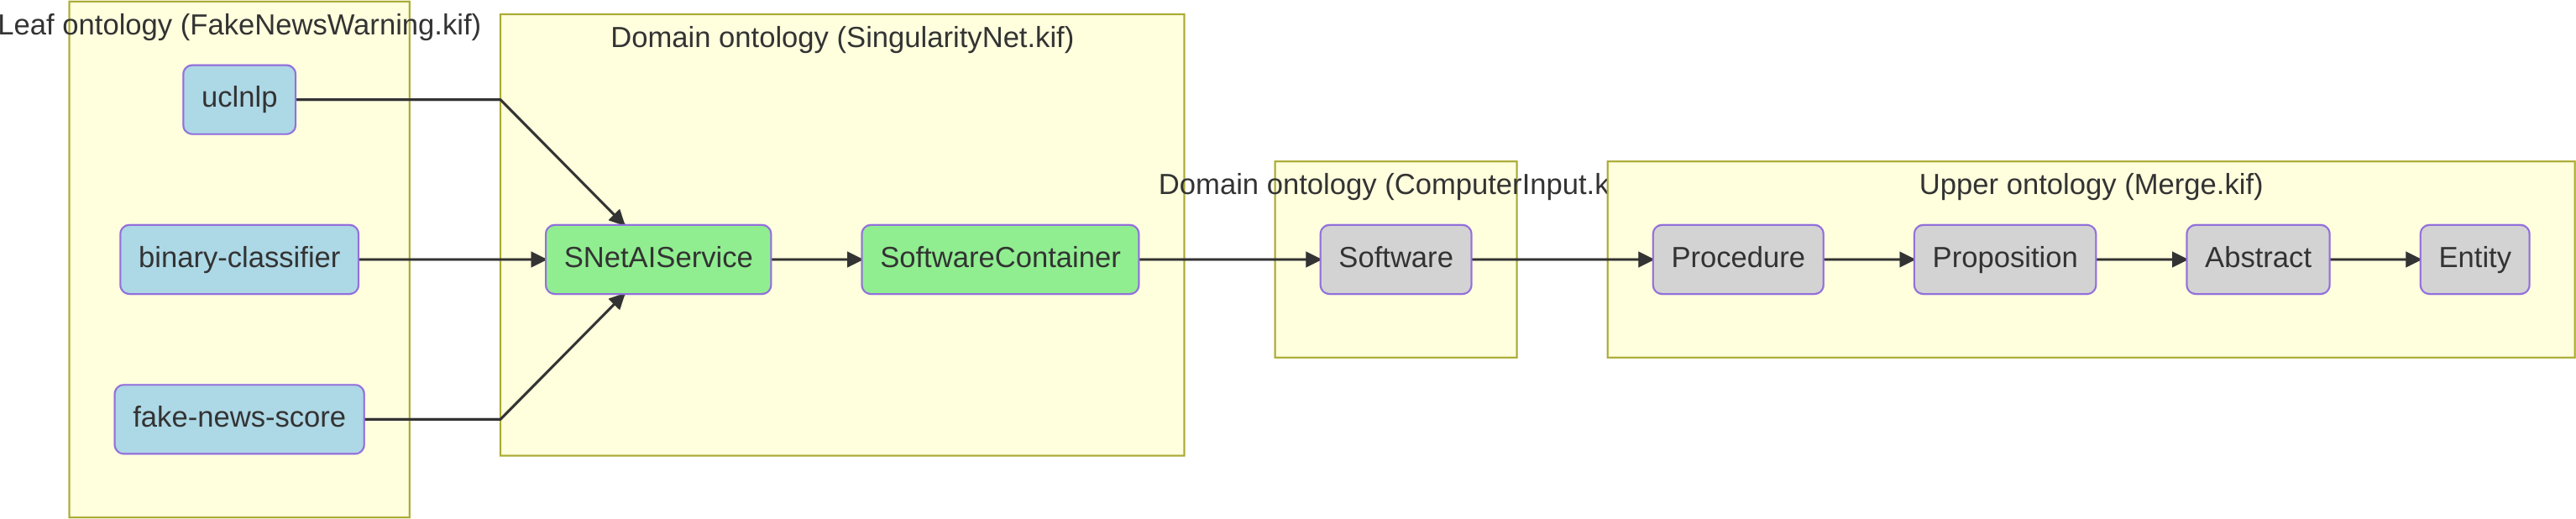
\includegraphics[width=\textwidth]{../../../ontology/images/SNetAIService.png}
		\caption{Class dependencies of the SNetAIService subclass within the ontology.}
		\label{fig:SNetAIService hierachy}
	\end{subfigure}
	\begin{subfigure}[b]{1\textwidth}
		\centering
		\includegraphics[width=\textwidth/4]{example-image-a}
		\caption{Class dependencies of the SNetAppBackend subclass (workflow definition) within the ontology.}
		\label{fig:tSNetAppBackend}
	\end{subfigure}
	\caption{Class dependences of AI-DSL Ontology (SingularityNet.kif) }
	\label{fig:SingularityNet.kif}
\end{figure}

\begin{figure}[h]
\inputminted[firstline=2, lastline=12, linenos,tabsize=2,breaklines, fontsize=\small]{scm}{../../../ontology/SingularityNet.kif}
\caption{\label{lst:singularitynet}Contents of SingularityNet.kif}
\end{figure}


\section{Future work}

\subsection{Combining ontology with Idris}

\kabir[inline]{It would be good to have a section explaining ideas about that, but I cannot do this alone, so probably the best is to reserve it for the end of the monht, when all the other aspects of AI-DSL project (including Idris) are explained.}




\chapter{Eman's work}

\chapter{Sam's work}



\bibliographystyle{splncs04}
\bibliography{local}

\end{document}
